\renewcommand{\thefigure}{\theenumi}
\renewcommand{\thetable}{\theenumi}
%%
%\begin{enumerate}[label=\thesection.\arabic*
%,ref=\thesection.\theenumi]

\subsection{Bernoulli to Gaussian}
\begin{enumerate}[label=\thesubsection.\arabic*
,ref=\thesection.\theenumi]


\item {\em Mean :}  The mean of the bernoulli distribution is 
\begin{align}
\mu = E\brak{X_i}  = \sum_{k=0}^{1}kp_{X_i}(k) = p = \frac{1}{6}
\end{align}
\item {\em Moment:}  The moment of the distribution is defined as
\begin{align}
E\brak{X_i^r}  = \sum_{k=0}^{1}k^rp_{X_i}(k) = p = \frac{1}{6}
\end{align}

%The second moment of the bernoulli distribution is 
%\begin{align}
%E\brak{X_i}  = \sum_{k=0}^{1}kp_{X_i}(k) = p = \frac{1}{6}
%\end{align}
\item {\em Variance :}  The variance of the bernoulli distribution is defined as
\begin{align}
\sigma^2 &= E\brak{X-E\brak{X}}^2  = E\brak{X^2}-E^2\brak{X} 
\\
&=p-p^2 = p\brak{1-p} = \frac{5}{36}
\end{align}
%
The standard deviation 
\begin{align}
\sigma =  \sqrt{p\brak{1-p}}
\end{align}
%
\item {\em The Gaussian Distribution: }  Define
\begin{align}
\label{eq:bern_gauss}
G = \frac{1}{\sqrt{n}}\sum_{k=1}^{n}\frac{X_i-\mu}{\sigma}
\end{align}
%
\item {\em Approximating Binomial Using Gaussian: } From \eqref{eq:bern_gauss}
and \eqref{eq:bern_binom},
%
\begin{align}
X & \approx \sigma\sqrt{n}G + n\mu 
\\
\implies F_X(k) &= \pr{\sigma\sqrt{n}G + n\mu  \le k }
\\
 &= F_G\brak{\frac{k-n\mu}{\sigma\sqrt{n}}} \approx \phi\brak{\frac{k-n\mu}{\sigma\sqrt{n}}} 
\label{eq:bern_gaussian_cdf}
\end{align}
where 
\begin{align}
\phi_{X}(x) = \int^{x}_{-\infty} \frac{1}{\sqrt{2\pi}}e^{-\frac{x^2}{2}}, -\infty < x < \infty
\end{align}
\item The 
probability density function (PDF) 
of $G$ is
%
\begin{align}
p_{G}(x) &= \frac{d}{dx}F_{X}(x)
\\
 &=  \frac{1}{{\sigma\sqrt{n}}}\phi^{\prime}\brak{\frac{k-n\mu}{\sigma\sqrt{n}}} 
\label{eq:bern_gaussian_pdf}
\end{align}
%
For large $n$, $G$ is a continuous distribution with probability density function (PDF)
\begin{align}
p_G(x) =  \frac{1}{\sqrt{2\pi}}\exp\brak{-\frac{x^2}{2}}, -\infty < x < \infty,
\end{align}
%
\item {\em Evaluationg the Probability: }  From \ref{eq:bern_gaussian_cdf}
and \ref{eq:bern_gaussian_pdf},
\begin{align}
\pr{X \le 1 } &= F_{G}(1) = p_G(0)+p_G(1) 
\\
&\approx 
0.41299463887797094
\label{eq:bern_gauss_ans}
\end{align}
which is close to \eqref{eq:bern_binom_ans}.
%
\end{enumerate}
\subsection{Uniform to Gaussian}
\begin{enumerate}[label=\thesubsection.\arabic*
,ref=\thesection.\theenumi]

\item
Generate $10^6$ samples of the random variable
%
\begin{equation}
X = \sum_{i=1}^{12}U_i -6
\end{equation}
%
using a C program, where $U_i, i = 1,2,\dots, 12$ are  a set of independent uniform random variables between 0 and 1
and save in a file called gau.dat
\\
\solution Download the following files and execute the  C program.
\begin{lstlisting}
codes/cdf/exrand.c
codes/cdf/coeffs.h
\end{lstlisting}

%
\item
Load gau.dat in python and plot the empirical CDF of $X$ using the samples in gau.dat. What properties does a CDF have?
\\
\solution The CDF of $X$ is plotted in Fig. \ref{fig:gauss_cdf}
\begin{figure}
\centering
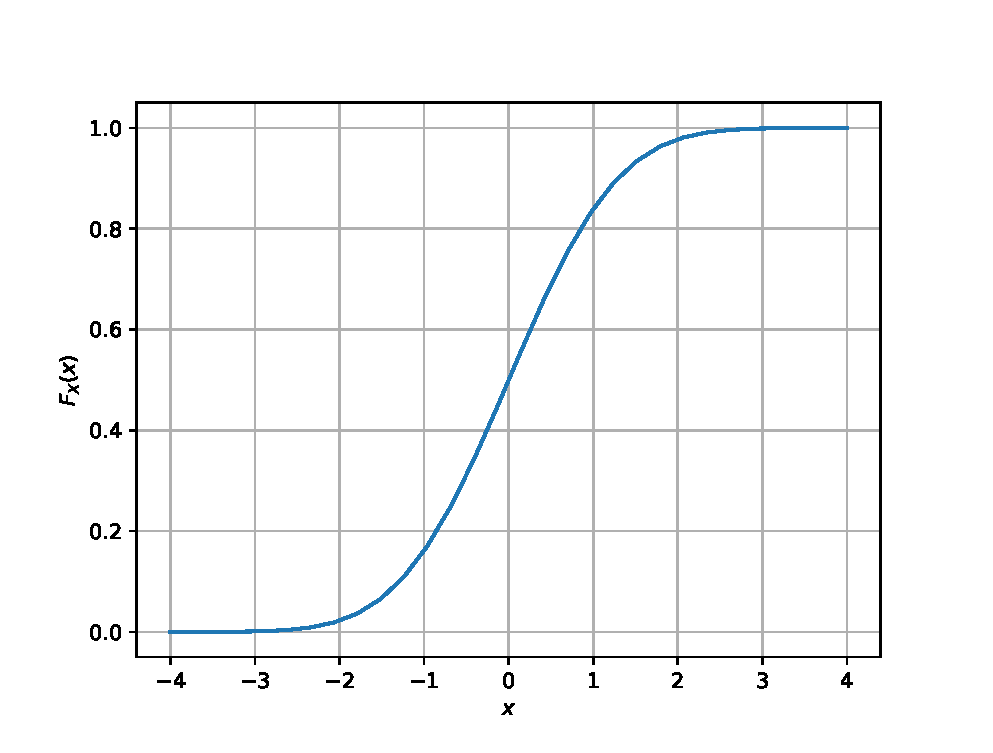
\includegraphics[width=\columnwidth]{./figs/clt/gauss_cdf}
\caption{The CDF of $X$}
\label{fig:gauss_cdf}
\end{figure}


\item
Load gau.dat in python and plot the empirical PDF of $X$ using the samples in gau.dat. The PDF of $X$ is defined as
\begin{align}
p_{X}(x) = \frac{d}{dx}F_{X}(x)
\end{align}
What properties does the PDF have?
\\
\solution The PDF of $X$ is plotted in Fig. \ref{fig:gauss_pdf} using the code below
\begin{lstlisting}
codes/clt/pdf_plot.py
\end{lstlisting}

\begin{figure}
\centering
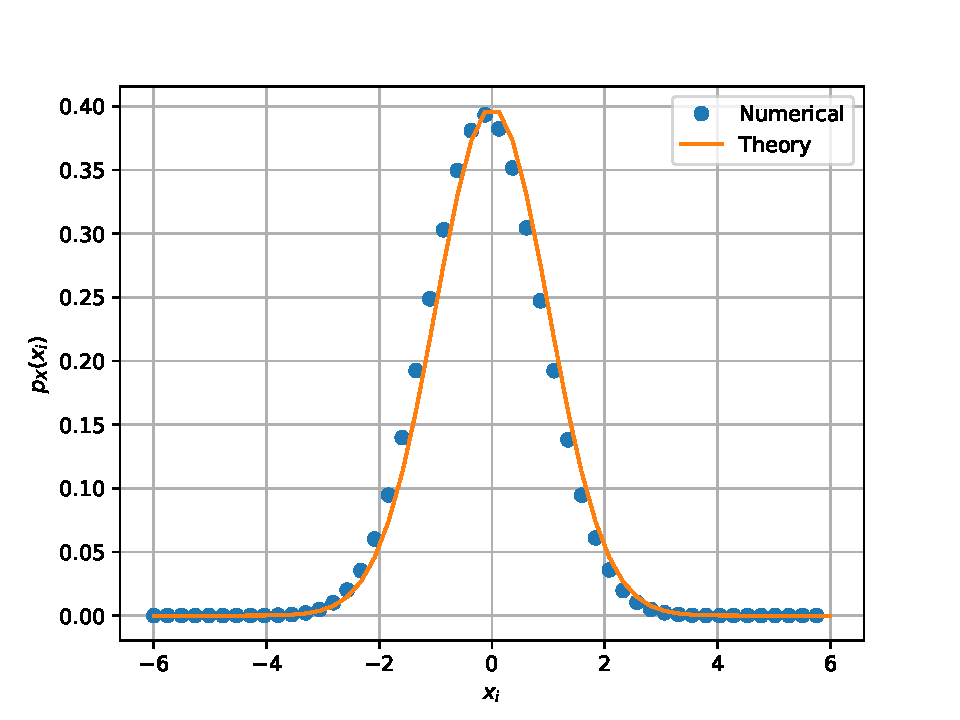
\includegraphics[width=\columnwidth]{./figs/clt/gauss_pdf}
\caption{The PDF of $X$}
\label{fig:gauss_pdf}
\end{figure}

\item Find the mean and variance of $X$ by writing a C program.
\\
\solution  Execute
\begin{lstlisting}
codes/clt/gaussian_numbers.c
\end{lstlisting}
\item Given that 
\begin{align}
p_{X}(x) = \frac{1}{\sqrt{2\pi}}\exp\brak{-\frac{x^2}{2}}, -\infty < x < \infty,
\label{eq:probman_gauss_pdf}
\end{align}
repeat the above exercise theoretically.
%
\\
\solution
The given curve 
\begin{align}
	y =\frac{1}{x-1}
\end{align}
can be expressed as 
\begin{align}
	xy - y - 1 = 0 \label{eq:solutions/1/14/eq:hyperbola}
\end{align}
Hence, we have
\begin{align}
	\vec{V} = \frac{1}{2}\myvec{0 & 1 \\ 1 & 0}, 
	\vec{u} = \frac{1}{2}\myvec{0 \\-1},
	f = -1
\end{align}
Since $\mydet{\vec{V}} < 0$, the equation \eqref{eq:solutions/1/14/eq:hyperbola} represents hyperbola.
To find the values of $\lambda_1$ and $\lambda_2$, consider the characteristic equation,
\begin{align}
	\mydet{\lambda\vec{I} - \vec{V}} &= 0\\
	\implies \mydet{\myvec{\lambda & 0\\0 & \lambda} - \myvec{0 & \frac{1}{2} \\ \frac{1}{2} & 0}} &= 0\\
	\implies \mydet{ \lambda & \frac{-1}{2} \\ \frac{-1}{2} & \lambda} &= 0\\
	\implies \lambda_1 &= \frac{1}{2} , \lambda_2 = \frac{-1}{2}
\end{align}
In addition, given the slope -1, the direction and normal vectors are given by 
\begin{align}
	\vec{m} = \myvec{1 \\ -1} \\
	\vec{n} = \myvec{ 1 \\ 1}
\end{align}
The parameters of hyperbola are as follows:
\begin{align}
	\vec{c} &= -\vec{V}^{-1}\vec{u} \\
	&= -\myvec{0 & 2\\ 2 & 0}\myvec{0 \\ -\frac{1}{2}} \\
	&= \myvec{1 \\ 0}\\
	axes &= \begin{cases}
	\sqrt{\frac{\vec{u}^T\vec{V}^{-1}\vec{u} - f}{\lambda_1}} = \sqrt{2}\\
 \sqrt{\frac{f-\vec{u}^T\vec{V}^{-1}\vec{u}}{\lambda_2}} = \sqrt{2}
\end{cases}
\end{align}
which represents the standard hyperbola equation,
\begin{align}
	\frac{x^2}{2} - \frac{x^2}{2} = 1
\end{align}
The points of contact are given by 
\begin{align}
  \tiny{K} &=\pm \sqrt{\frac{\vec{u}^T\vec{V}^{-1}\vec{u} - f}{\vec{n}^T\vec{V}^{-1}\vec{n}}}
  = \pm \frac{1}{2}\\
  \vec{q} &= \vec{V}^{-1}(k\vec{n}-\vec{u})\\
  \vec{q_1} &= \myvec{0 & 2\\2 & 0} \sbrak{\frac{1}{2}\myvec{1 \\ 1} - \myvec{0\\ \frac{-1}{2}}}\\
  &= \myvec{2 \\ 1}\\
  \vec{q_2} &= \myvec{0 & 2\\2 & 0} \sbrak{\frac{-1}{2}\myvec{1 \\ 1} - \myvec{0\\ \frac{-1}{2}}}\\
  &= \myvec{0 \\ -1}
\end{align} 
$\therefore$ The tangents are given by
\begin{align}
	\myvec{1 & 1} \brak{\vec{x} - \myvec{2 \\ 1}} = 0 \\
	\myvec{1 & 1} \brak{\vec{x} - \myvec{0 \\ -1}} = 0
\end{align}
The desired equations of all lines having slope -1 that are tangents to the curve $\frac{1}{x-1}, x \neq 1$ are given by
\begin{align}
	\myvec{1 & 1}\vec{x} &= 3 \\
	\myvec{1 & 1}\vec{x} &= -1 
\end{align}
The above results are verified in the following figure.
\begin{figure}[h!] \label{eq:solutions/1/14/fig:tangents}
	\centering
	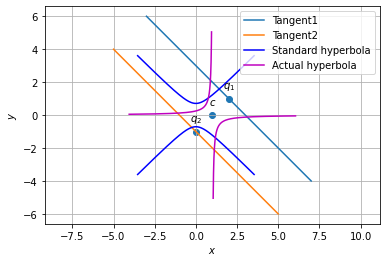
\includegraphics[width=\columnwidth]{./solutions/1/14/graph7.png}
	\caption{The standard and actual hyperbola.}
\end{figure}

\item Let $U$ be a uniform random variable between 0 and 1.
%\begin{enumerate}[label=\thesection.\arabic*
%,ref=\thesection.\theenumi]

%
\item
Load the uni.dat file into python and plot the empirical CDF of $U$ using the samples in uni.dat. The CDF is defined as
\begin{align}
F_{U}(x) = \pr{U \le x}
\end{align}
\\
\solution  The following code plots Fig. \ref{fig:uni_cdf}
\begin{lstlisting}
codes/cdf/cdf_plot.py
\end{lstlisting}
\begin{figure}
\centering
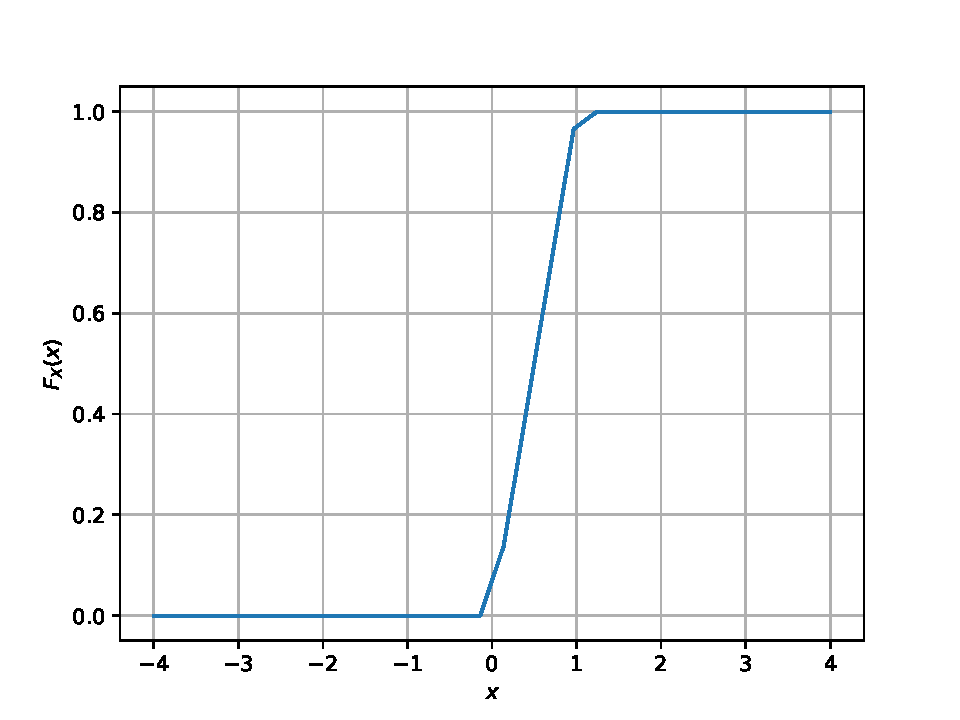
\includegraphics[width=\columnwidth]{./figs/cdf/uni_cdf}
\caption{The CDF of $U$}
\label{fig:uni_cdf}
\end{figure}

%\item Generate $10^6$ samples of $U$ using a C program and save into a file called uni.dat .
%\\


%
\item
Find a  theoretical expression for $F_{U}(x)$.

\item
The mean of $U$ is defined as
%
\begin{equation}
E\sbrak{U} = \frac{1}{N}\sum_{i=1}^{N}U_i
\end{equation}
%
and its variance as
%
\begin{equation}
\text{var}\sbrak{U} = E\sbrak{U- E\sbrak{U}}^2 
\end{equation}

Write a C program to  find the mean and variance of $U$. 
\item Verify your result theoretically given that
%
\begin{equation}
E\sbrak{U^k} = \int_{-\infty}^{\infty}x^kdF_{U}(x)
\end{equation}

\end{enumerate}



